%%%%%%%%%%%%%%%%%%%%%%%%%%%%%%%%%%%%%%%%%
% Short Sectioned Assignment LaTeX Template Version 1.0 (5/5/12)
% This template has been downloaded from: http://www.LaTeXTemplates.com
% Original author:  Frits Wenneker (http://www.howtotex.com)
% License: CC BY-NC-SA 3.0 (http://creativecommons.org/licenses/by-nc-sa/3.0/)
%%%%%%%%%%%%%%%%%%%%%%%%%%%%%%%%%%%%%%%%%

%----------------------------------------------------------------------------------------
%	PACKAGES AND OTHER DOCUMENT CONFIGURATIONS
%----------------------------------------------------------------------------------------

\documentclass[paper=a4, fontsize=11pt]{scrartcl} % A4 paper and 11pt font size

% ---- Entrada y salida de texto -----

\usepackage[T1]{fontenc} % Use 8-bit encoding that has 256 glyphs
\usepackage[utf8]{inputenc}
%\usepackage{fourier} % Use the Adobe Utopia font for the document - comment this line to return to the LaTeX default

% ---- Idioma --------

\usepackage[spanish, es-tabla]{babel} % Selecciona el español para palabras introducidas automáticamente, p.ej. "septiembre" en la fecha y especifica que se use la palabra Tabla en vez de Cuadro

% ---- Otros paquetes ----

\usepackage{amsmath,amsfonts,amsthm} % Math packages
%\usepackage{graphics,graphicx, floatrow} %para incluir imágenes y notas en las imágenes
\usepackage{graphics,graphicx, float, url} %para incluir imágenes y colocarlas

% Para hacer tablas comlejas
%\usepackage{multirow}
%\usepackage{threeparttable}
\usepackage{float}


%\usepackage{sectsty} % Allows customizing section commands
%\allsectionsfont{\centering \normalfont\scshape} % Make all sections centered, the default font and small caps

\usepackage{fancyhdr} % Custom headers and footers
\pagestyle{fancyplain} % Makes all pages in the document conform to the custom headers and footers
\fancyhead{} % No page header - if you want one, create it in the same way as the footers below
\fancyfoot[L]{} % Empty left footer
\fancyfoot[C]{} % Empty center footer
\fancyfoot[R]{\thepage} % Page numbering for right footer
\renewcommand{\headrulewidth}{0pt} % Remove header underlines
\renewcommand{\footrulewidth}{0pt} % Remove footer underlines
\setlength{\headheight}{13.6pt} % Customize the height of the header

\numberwithin{equation}{section} % Number equations within sections (i.e. 1.1, 1.2, 2.1, 2.2 instead of 1, 2, 3, 4)
\numberwithin{figure}{section} % Number figures within sections (i.e. 1.1, 1.2, 2.1, 2.2 instead of 1, 2, 3, 4)
\numberwithin{table}{section} % Number tables within sections (i.e. 1.1, 1.2, 2.1, 2.2 instead of 1, 2, 3, 4)

\setlength\parindent{0pt} % Removes all indentation from paragraphs - comment this line for an assignment with lots of text

\newcommand{\horrule}[1]{\rule{\linewidth}{#1}} % Create horizontal rule command with 1 argument of height


\title{	
	\normalfont \normalsize 
	\textsc{{\bf Ingeniería de Servidores (2015-2016)} \\ Grado en Ingeniería Informática y Matemáticas \\ Universidad de Granada} \\ [25pt] % Your university, school and/or department name(s)
	\horrule{0.5pt} \\[0.4cm] % Thin top horizontal rule
	\huge Memoria Práctica 3 \\ % The assignment title
	\horrule{2pt} \\[0.5cm] % Thick bottom horizontal rule
}

\author{Iván Sevillano García} % Nombre y apellidos

\date{\normalsize\today} % Incluye la fecha actual

\begin{document}

\maketitle % Muestra el Título

\newpage %inserta un salto de página

\tableofcontents % para generar el índice de contenidos

\newpage

\section{Conociendo el subsistema de archivos.}

\subsection{Cuestión 1:}

\begin{itemize}
	\item \textbf{¿Qué archivo le permite ver qué programas se han instalado con el gestor de paquetes?}\\
	En el directorio $/var/log/apt/$,donde se encuentran los archivos history.log y term.log. Además, encontramos también archivos con los mismos nombres con las extensiones que abajo se especifican(donde podemos encontrar cualquier número como extensión).
	
	\item \textbf{¿Qué significan las terminaciones .1.gz o .2.gz de los archivos en ese directorio?}\\
	Cada vez que llenamos lo suficiente nuestro archivo history.log, el sistema la comprime y crea un nuevo history.log para almacenar la información sobre nuevos paquetes que instalemos. Las extensiones con distinto número no son más que formas de numerar los distintos paquetes por orden. El orden que siguen va desde el más reciente (extensión .1.gz) hasta el más antiguo.
	
\end{itemize}

\subsection{Programación de tareas con cron}
\begin{itemize}
	\item \textbf{¿Qué archivo ha de modificar para programar una tarea? Escriba la línea
		necesaria para ejecutar una vez al día una copia del directorio ~/codigo a ~/seguridad/
		$fecha$ donde $fecha$ es la fecha actual (puede usar el comando date)}\\
	Según \cite{crontab}, debemos modificar los archivos en $/var/spool/cron/crontabs/$, sin embargo no están hechos para ser modificados directamente. Se nos ofrece, para modificar el archivo de programación de tareas, el comando $crontab$, que con la opción $-e$, nos deja modificar desde la terminal con el editor de texto que prefiramos.\\
	
	La linea que debemos añadir será la siguiente:\\
	
	$0 0 * * * cp -r ~codigo ~/seguridad/`date`$\\
	
	Los primeros cinco $items$ de la sentencia indican cuando queremos que se realice la tarea que se muestra a continuación, por este orden: minuto hora diaDelMes Mes DiaDeLaSemana. No hace especificar todos los campos, ya que el poner un asterisco($*$) nos dice que no tenga en cuenta este campo. Por ello, en nuestra sentencia, queremos que se ejecute el comando siempre que sean las doce de la noche, sea el día que sea, el mes que sea y el día de la semana que sea.
\end{itemize}

\section{Analizando que ocurre en el Kernel con Dmesg}

\begin{itemize}
	\item \textbf{Pruebe a ejecutar el comando, conectar un dispositivo USB y vuelva a
		ejecutar el comando. Copie y pegue la salida del comando (considere usar dmesg |
		tail). Comente qué observa en la información mostrada.}\\
	
	\begin{figure}[H]
	\centering
	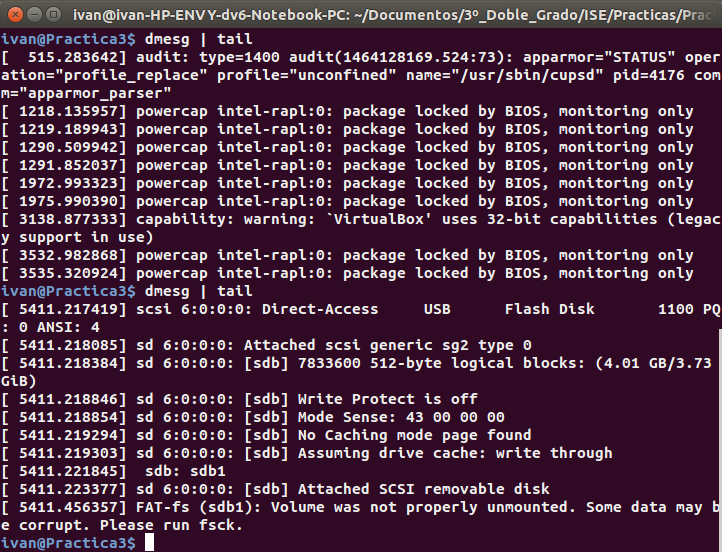
\includegraphics[width=0.7\linewidth]{dmesgPenDrive}
	\caption[dmesg]{Mensaje mostrado por dmesg antes y después de conectar un pen-drive}
	\label{fig:dmesgPenDrive}
	\end{figure}
	
	Antes de conectar el pen-drive, no teníamos ninguna referencia del mismo. Tras conectarlo, el primer mensaje que se nos muestra es la presencia del mismo. También nos ofrece más información como que el disco no fue debidamente desmontado.

	
\end{itemize}



\newpage
\begin{thebibliography}{xx}
	\bibitem{crontab} http://linux.die.net/man/1/crontab
	
\end{thebibliography}
\end{document}